% Chapter 2

\chapter{Introducción Específica} % Main chapter title

\label{Chapter2} 
\label{IntroEsp}

%----------------------------------------------------------------------------------------

En este capítulo se explorarán en términos muy generales las distintas tecnologías, arquitecturas, paradigmas y técnicas que resultaron útiles para el desarrollo del trabajo.


\section{Seguimiento Ocular (Eye-tracking)}

El \emph{eye-tracking}, que se traduce literalmente como \emph{seguimiento ocular}, es el proceso tecnológico que permite medir y registrar el punto de la mirada de una persona o el movimiento de sus ojos en relación con la cabeza. Para ello, comúnmente se utiliza como punto de referencia el centro de la pupila. A diferencia del seguimiento facial (que analiza músculos, cejas o expresiones), el \emph{eye-tracking} se concentra estrictamente en la forma y movimientos del globo ocular (Fig. \ref{fig:eyetracking}).

\begin{figure}[htbp]
    \centering
    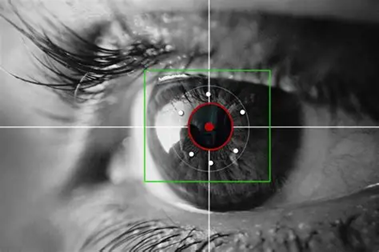
\includegraphics[width=0.3\textwidth]{figuras/eyetracking.png}
    \caption{Representación gráfica del Eye-Tracking}
    \label{fig:eyetracking}
\end{figure}

Si bien esta tecnología cuenta con décadas de investigación y ha sido ampliamente utilizada en laboratorios de psicología, neuromarketing y análisis de usabilidad, el desarrollo de hardware más accesible ha permitido expandir sus aplicaciones. Una de estas aplicaciones directas es la \emph{interacción basada en la mirada} (\emph{gaze interaction}), donde los datos del movimiento ocular se utilizan para manipular un entorno digital. 

En el caso del presente trabajo, orientado a la inclusión en el ámbito educativo, se implementa el seguimiento ocular enfocado en detectar hacia cuál de las opciones disponibles está dirigiendo la mirada el alumno. Esta información se procesa para registrar la selección correspondiente, permitiéndole responder cuestionarios de opción múltiple sin necesidad de manipular un cursor en pantalla ni requerir destreza física.

\section{Procesamiento de Imágenes y Visión por Computadora}

Para poner en práctica la disciplina del \emph{Eye-Tracking} existen muchas maneras. En esta sección se describirá una técnica de visión computacional llamada \emph{Coincidencia de patrones} o \emph{Template Matching}, y \emph{OpenCV}, una librería fundamental para su implementación.

\subsection{Conceptos fundamentales y biblioteca OpenCV}
El procesamiento de imágenes puede definirse como el proceso mediante el cual se modifica una imagen de entrada para obtener otra distinta mediante algoritmos matemáticos (ya sea para aumentar o disminuir su resolución, recortarla o cambiar su paleta de colores, entre otros procedimientos). En este contexto, dichas modificaciones se realizan con el fin de acondicionar la imagen para posteriores análisis computacionales.

Por otro lado, la visión computacional es el análisis que realiza una máquina sobre una imagen (usualmente procesada con anterioridad), con el fin de extraer características, interpretarlas y aprender de ellas, simulando la percepción visual humana. El \emph{Eye-Tracking}, descrito en secciones anteriores, es un claro ejemplo de un proceso de visión computacional.

Lograr que una máquina interprete de manera autónoma el comportamiento de las imágenes es una tarea compleja, motivo por el cual se emplean herramientas especializadas que facilitan el proceso. Una de las más destacadas es \emph{OpenCV (Open Source Computer Vision Library)}, la biblioteca de código abierto más popular e importante en el campo del análisis visual. Fue creada por la empresa \emph{Intel} y cuenta con más de 2500 algoritmos matemáticos optimizados que sirven tanto para el procesamiento de imágenes como para la visión computacional. Entre sus principales capacidades destacan la manipulación estructural, la detección de características geométricas (como bordes, esquinas o líneas), la coincidencia de patrones, la detección de objetos y el análisis de movimiento.

\subsection{Coincidencia de patrones (Template Matching)}
La coincidencia de patrones, conocida en inglés como \emph{Template Matching}, es una técnica de visión computacional diseñada para buscar y encontrar la ubicación de una imagen pequeña (denominada plantilla o molde) dentro de una imagen de mayor tamaño.

El proceso funciona deslizando la plantilla píxel por píxel sobre la imagen principal, de izquierda a derecha y de arriba hacia abajo. En cada posición evaluada, el algoritmo utiliza una fórmula matemática para calcular un puntaje de similitud entre la plantilla original y el fragmento de la imagen principal que se está superponiendo en ese instante.

El resultado de esta operación no es una imagen, sino una matriz bidimensional de resultados. El punto con el valor estadístico más alto indica la coordenada exacta donde el algoritmo encontró la mayor coincidencia geométrica.


\section{Redes Neuronales Artificiales}

\subsection{Definición y conceptos básicos}

Para comprender este concepto es necesario definir previamente el \emph{Machine Learning (ML)} o \emph{Aprendizaje automático}. Esta rama de las ciencias de la computación permite a los sistemas aprender y resolver problemas sin ser programados de forma tradicional, suministrando datos a una computadora para que construya un modelo predictivo basado en esa experiencia (Fig. \ref{fig:machinelearning}).

\begin{figure}[htbp]
\centering
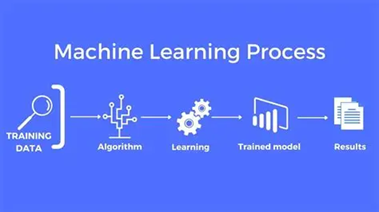
\includegraphics[width=0.5\textwidth]{figuras/machinelearning.png}
\caption{El proceso del \emph{Machine Learning}}
\label{fig:machinelearning}
\end{figure}

Dentro de los modelos de ML, uno de los más eficaces son las Redes Neuronales Artificiales. Reciben este nombre debido a que su estructura (basada en celdas o nodos interconectados para el procesamiento de información) se inspira directamente en el comportamiento biológico del sistema nervioso.

\subsection{Principio de funcionamiento}

Estas redes organizan sus neuronas en tres niveles jerárquicos principales: la capa de entrada (recibe los datos en crudo, como los píxeles de una imagen), las capas ocultas (el núcleo de procesamiento que detecta desde características básicas hasta patrones complejos) y la capa de salida (que entrega el resultado final, como las coordenadas de una pupila) (Fig. \ref{fig:redneuronal}).

\begin{figure}[htbp]
\centering
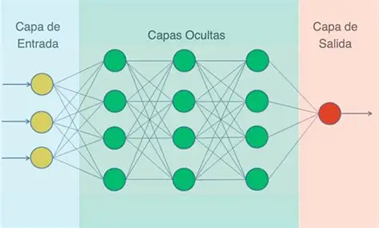
\includegraphics[width=0.5\textwidth]{figuras/redneuronal.png}
\caption{Diagrama simplificado de una red neuronal}
\label{fig:redneuronal}
\end{figure}

El aprendizaje del modelo se logra mediante el entrenamiento, un proceso iterativo donde la red evalúa datos conocidos y ajusta su matemática interna para minimizar el margen de error. Durante estos ciclos, cada neurona ejecuta una ecuación fundamental:

\begin{equation}
z = \sum w_i x_i + b
\end{equation}

Donde $xi$ representa el dato de entrada individual, $w_i$ es el peso (la importancia relativa asignada a esa entrada específica) y \emph{b} es el sesgo o bias (una constante de adaptación algorítmica). El resultado \emph{z} es evaluado finalmente por una función de activación, la cual determina con qué intensidad la neurona transmite la señal hacia la siguiente capa.

\subsection{Tipos y arquitecturas de redes}

La arquitectura del modelo varía estrictamente según la naturaleza del problema a resolver. Se distinguen tres categorías fundamentales:

\begin{itemize}

\item Prealimentadas (\emph{Feedforward}): La información viaja de forma unidireccional (de entrada a salida). Son ideales para problemas sencillos con datos livianos que no requieren memoria temporal.

\item Convolucionales (\emph{CNN}): Utilizan filtros matemáticos para analizar los datos espaciales por secciones. Son la arquitectura por excelencia para procesar imágenes y video en tiempo real.

\item Recurrentes (\emph{RNN}): Poseen bucles internos que les otorgan memoria secuencial, perfectas para contextos de análisis temporal (como procesamiento de lenguaje natural o secuencias largas de video).

Dado que este proyecto requiere analizar la posición espacial de las pupilas en un flujo de video en tiempo real, y considerando que se puede prescindir del contexto temporal (memoria secuencial), se concluye que la arquitectura a implementar en este dispositivo es una Red Neuronal Convolucional.

\end{itemize}

\section{Sistemas Embebidos y Control Gráfico}

\subsection{Microcontroladores y microprocesadores}

En el diseño de sistemas embebidos actuales, la optimización de costos, espacio y consumo energético recae fundamentalmente en la implementación de microprocesadores y microcontroladores. 

Un microprocesador (MPU) constituye la unidad central de procesamiento de un sistema. Se trata de un circuito integrado encargado de decodificar y ejecutar instrucciones aritméticas y lógicas. Su arquitectura interna se compone de una Unidad Aritmético Lógica (ALU), registros de memoria ultrarrápida y buses de datos y control que transmiten señales eléctricas binarias. Al carecer de memoria masiva y periféricos integrados, requiere de componentes externos interconectados en una placa base para conformar un sistema funcional. 

Por otro lado, un microcontrolador (MCU) es un sistema informático completo encapsulado en un único circuito integrado. Su estructura integra un microprocesador central junto con bloques de memoria interna (tanto volátil para datos como no volátil para el programa) y múltiples periféricos. Estos módulos adicionales pueden incluir conversores analógico-digitales (ADC) y digital-analógicos (DAC), temporizadores, protocolos de comunicación serial y puertos de entrada/salida de propósito general (GPIO), lo que le permite interactuar directamente con el entorno físico y dispositivos externos de manera autónoma. 

Un ejemplo sumamente conocido de microcontroladores es la placa de desarrollo \emph{Arduino Uno} (Fig. \ref{fig:arduinouno})

\begin{figure}[H]
    \centering
    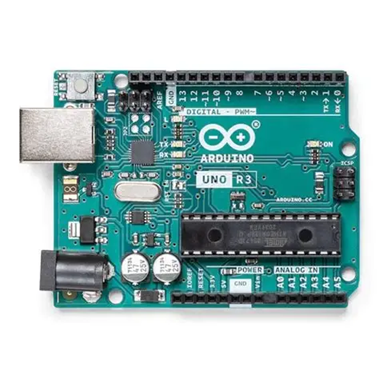
\includegraphics[width=0.5\textwidth]{figuras/arduinouno.png}
    \caption{Placa de desarrollo \emph{Arduino Uno}}
    \label{fig:arduinouno}
\end{figure}

\subsection{Familia de microcontroladores ESP32}

Otro modelo del placas de desarrollo que ha ganado enorme popularidad en el desarrollo de sistemas embebidos y el Internet de las Cosas (IoT) es el microcontrolador ESP32. Creado por la compañía Espressif Systems, este dispositivo surgió como una solución de bajo costo y alta eficiencia energética diseñada para suplir la creciente necesidad de conectividad inalámbrica en proyectos electrónicos. A diferencia de las placas más tradicionales, el ESP32 destaca por integrar módulos de Wi-Fi y Bluetooth (tanto clásico como de baja energía) directamente dentro del mismo chip.

Además de sus excelentes capacidades de comunicación, este microcontrolador representa un salto significativo en cuanto a potencia computacional. Al estar generalmente equipado con un procesador de doble núcleo y una memoria considerablemente mayor que la de sus predecesores, permite manejar tareas más complejas, alojar servidores web locales y procesar datos a mayor velocidad. Gracias a este equilibrio entre rendimiento, conectividad y tamaño reducido, el ESP32 se ha convertido en una pieza fundamental para la ingeniería de dispositivos modernos e interconectados.

\subsection{Interfaces gráficas embebidas y biblioteca LVGL}

El desarrollo de interfaces gráficas de usuario (GUI, por sus siglas en inglés) en sistemas embebidos presenta desafíos asociados a las restricciones de memoria RAM, capacidad de cómputo y consumo de energía de los microcontroladores. A diferencia de los entornos convencionales, donde el sistema operativo gestiona los recursos visuales mediante unidades de procesamiento gráfico dedicadas (GPU), en un microcontrolador el renderizado debe ejecutarse de forma eficiente para garantizar fluidez visual y respuesta táctil en tiempo real sin sobrecargar la CPU.

Para resolver esta problemática, se recurre a bibliotecas gráficas optimizadas para hardware limitado, entre las que destaca \textbf{LVGL} (\emph{Light and Versatile Graphics Library}). LVGL es una biblioteca de código abierto escrita en lenguaje C, diseñada para operar con requerimientos mínimos de memoria. Implementa un modelo orientado a objetos basado en elementos visuales predefinidos (\emph{widgets}) como botones, etiquetas, listas, deslizadores y contenedores, los cuales pueden personalizarse mediante estilos y animaciones.

La arquitectura de LVGL se fundamenta en el desacoplamiento entre la lógica de la interfaz y el hardware subyacente. Esto se logra a través de dos componentes principales:
\begin{itemize}
    \item Controlador de pantalla (\emph{Display Driver}): transfiere los píxeles renderizados desde el búfer de dibujo interno de la biblioteca hacia el controlador físico del panel (por ejemplo, a través de interfaces SPI o paralelas), admitiendo técnicas de doble búfer (\emph{double buffering}) para evitar parpadeos en pantalla.
    \item Controlador de dispositivo de entrada (\emph{Input Device Driver}): gestiona la lectura y calibración de periféricos interactivos, como pantallas táctiles resistivas o capacitivas, teclados y codificadores rotativos.
\end{itemize}

En el ámbito del hardware comercial de bajo costo, esta combinación de pantalla, interfaz táctil y microcontrolador suele integrarse en módulos compactos denominados comúnmente \emph{Cheap Yellow Display} (CYD), los cuales incorporan un SoC ESP32 junto con un panel TFT y un controlador táctil resistivo (típicamente XPT2046) interconectados mediante bus SPI. La integración de LVGL sobre estas plataformas permite ejecutar interfaces interactivas fluidas directamente en el dispositivo embebido de manera autónoma.

\begin{figure}[htbp]
    \centering
    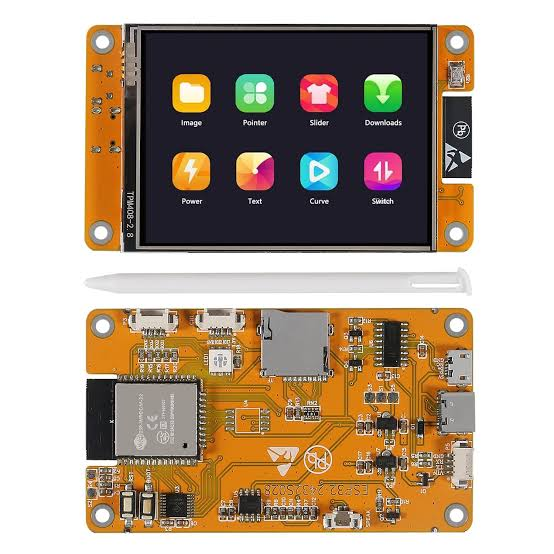
\includegraphics[width=0.5\textwidth]{figuras/esp32cyd.png}
    \caption{Placa de desarrollo \emph{ESP32-CYD} (vista frontal y trasera)}
    \label{fig:esp32cyd}
\end{figure}

\section{Redes y Comunicaciones}

\subsection{Redes locales Wi-Fi}

El estándar IEEE 802.11, conocido comúnmente como Wi-Fi, define los protocolos para la implementación de redes de área local inalámbricas (WLAN). La topología de estas redes se estructura a través de dos modos de operación:

\begin{itemize}
    \item Modo Estación (\emph{Station} - STA): en esta configuración, el nodo inalámbrico actúa como cliente. Su función consiste en explorar el espectro de radiofrecuencia, detectar una red existente a través de su identificador (SSID), autenticarse mediante los protocolos de seguridad correspondientes (como WPA2/WPA3) y asociarse a un punto de acceso central para integrarse al tráfico de dicha red.
    \item Modo Punto de Acceso (\emph{Access Point} - AP o SoftAP): en este modo, el dispositivo asume el rol de concentrador e iniciador de la red. Es el encargado de emitir periódicamente tramas de sincronización (\emph{beacon frames}) para anunciar la presencia de la red, autenticar a los nodos que solicitan conexión y gestionar la tabla de clientes asociados, de esta manera crea una infraestructura de red local independiente.
\end{itemize}

En el marco de este trabajo, uno de los módulos del sistema se configura en modo Access Point para generar una red local cerrada e independiente, mientras que tanto el módulo de captura de imagen como los dispositivos de los usuarios se conectan a dicha red en modo Station, permitiendo la comunicación directa entre todos los componentes sin depender de un router externo ni de acceso a internet.

\begin{figure}[htbp]
    \centering
    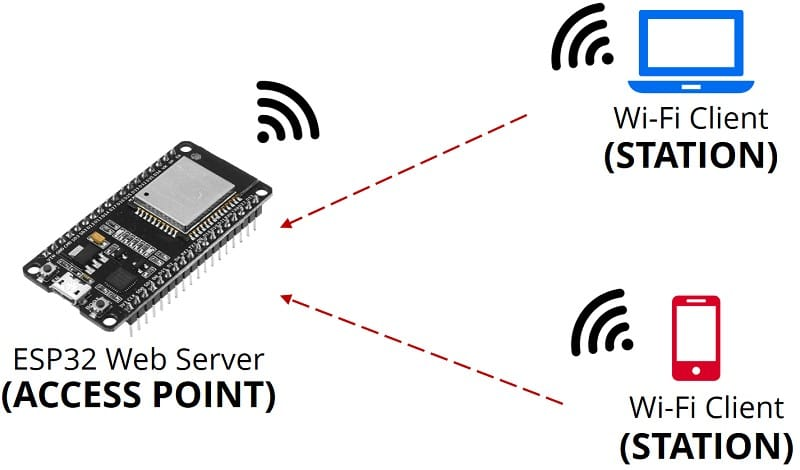
\includegraphics[width=0.5\textwidth]{figuras/esp32wifi.png}
    \caption{Red Wi-Fi con un microcontrolador ESP32 actuando como punto de acceso}
    \label{fig:esp32wifi}
\end{figure}

\subsubsection{Direccionamiento IP y transmisión de datos}

La comunicación en una red de datos se rige por protocolos que definen cómo se estructura, transmite y recibe la información. Dentro de estas reglas, el direccionamiento lógico permite identificar a cada dispositivo de manera unívoca para asegurar que los datos alcancen su destino.

\begin{itemize}
    \item Protocolo IP (\textit{Internet Protocol}): estructura los datos en paquetes que contienen las direcciones de origen y destino para su entrega en la red. En redes locales bajo la versión IPv4, la dirección de cada dispositivo se establece mediante dos modalidades:
    \begin{itemize}
        \item Asignación estática: la dirección se define de manera manual en el equipo y permanece fija a lo largo del tiempo, lo que permite localizar siempre al dispositivo en esa misma dirección.
        \item Asignación dinámica: el protocolo de configuración dinámica de host (DHCP, \textit{Dynamic Host Configuration Protocol}) asigna una dirección disponible de forma automática al asociarse el equipo a la red, lo que agiliza la incorporación de nuevos dispositivos sin requerir configuraciones individuales.
    \end{itemize}

    \item Protocolo HTTP (\textit{Hypertext Transfer Protocol}): opera bajo el modelo cliente-servidor mediante un esquema de peticiones y respuestas. Para asegurar que la información no sufra pérdidas ni alteraciones en su secuencia, HTTP utiliza TCP (\textit{Transmission Control Protocol}), el cual establece una conexión confiable previa al intercambio de datos. Mediante este mecanismo se transfieren páginas web, estilos y datos estructurados.

    \item Transmisión continua de video (\textit{Streaming} MJPEG): en lugar de realizar una petición HTTP por cada imagen, la técnica MJPEG (\textit{Motion} JPEG) mantiene una única conexión abierta para enviar una secuencia continua de fotogramas JPEG independientes delimitados por un separador. El cliente actualiza la imagen en pantalla a medida que recibe cada cuadro, logrando una visualización de video fluida en tiempo real.
\end{itemize}

\section{Arquitectura y Patrones de Software}

\subsection{Modelo Cliente/Servidor}

La arquitectura cliente/servidor (Fig. \ref{fig:clienteservidor}) es un modelo de diseño de software y redes en el cual las tareas a realizar se distribuyen entre un proveedor de recursos o servicios denominado “Servidor” y un receptor o demandante de dichos servicios denominado “Cliente”. Se basa en una dinámica de petición/respuesta entre ambas entidades. Sus componentes principales son:

\begin{itemize}

\item El \keyword{cliente}: Es el dispositivo o aplicación que interactúa con el usuario final. Su función principal es la de elaborar y enviar peticiones de datos o ejecución de tareas a través de una red, y luego recibir, formatear y presentar los resultados obtenidos en la interfaz de usuario. Es el componente que siempre inicia la comunicación.

\item El \keyword{servidor}: Es el dispositivo o programa en ejecución continua diseñado para escuchar, recibir y procesar las peticiones de uno o múltiples clientes. Su función es la de administrar los recursos y servicios para devolver al cliente la respuesta solicitada.

%       \item La \keyword{red} y los \keyword{protocolos}: La red es la vía física o inalámbrica por la cual se comunican los dispositivos (generalmente internet), mientras que los protocolos son el conjunto de reglas o parámetros que estos dispositivos cumplen para que la comunicación sea efectiva.

\end{itemize}

Esta forma de trabajo es muy utilizada en los sistemas embebidos modernos para centralizar la carga de trabajo en un único dispositivo (el servidor), en lugar de que cada uno de los clientes tenga su propia base de datos y recursos, lo cual incrementaría significativamente los costos y la complejidad de hardware en cada terminal, volviendo los procesos ineficientes. 

\begin{figure}[htbp]
    \centering
    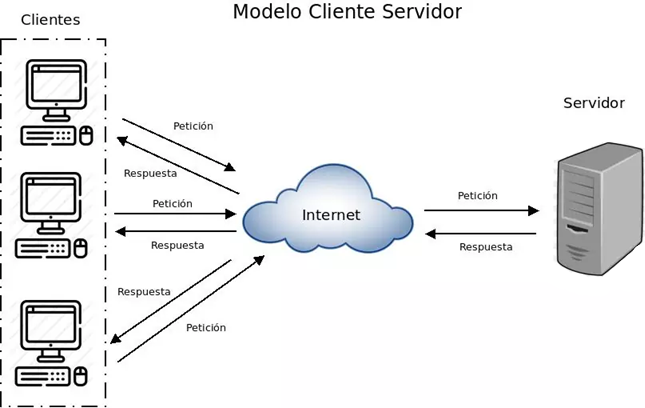
\includegraphics[width=0.5\textwidth]{figuras/clienteservidor.png}
    \caption{El sistema \emph{Cliente/Servidor}}
    \label{fig:clienteservidor}
\end{figure}

\subsection{Patrón de diseño Modelo-Vista-Controlador (MVC)}

El patrón Modelo-Vista-Controlador (\emph{Model-View-Controller} - MVC) es una estrategia de diseño de software orientada a desacoplar la lógica de negocio, la gestión de datos y la interfaz de usuario en tres componentes con responsabilidades bien definidas:

\begin{itemize}
    \item Modelo (\emph{Model}): representa la estructura de los datos del sistema y gestiona las reglas de negocio. Se encarga de interactuar con los mecanismos de almacenamiento y persistencia para consultar, insertar, modificar o eliminar registros, asegurando la integridad de la información sin vincularse con la interfaz gráfica.
    \item Vista (\emph{View}): constituye la capa de presentación con la que interactúa el usuario. Su función es recibir los datos procesados y renderizarlos en un formato comprensible, capturando los eventos y acciones del usuario para transferirlos al controlador.
    \item Controlador (\emph{Controller}): actúa como intermediario entre el modelo y la vista. Procesa las solicitudes y eventos originados en la vista, ejecuta la lógica correspondiente, solicita las operaciones necesarias al modelo y actualiza la vista con el resultado.
\end{itemize}

Esta separación de responsabilidades favorece la modularidad, simplifica el mantenimiento del sistema y permite modificar la interfaz visual o el almacenamiento de datos de forma independiente sin alterar la lógica central de la aplicación.

\begin{figure}[htbp]
    \centering
    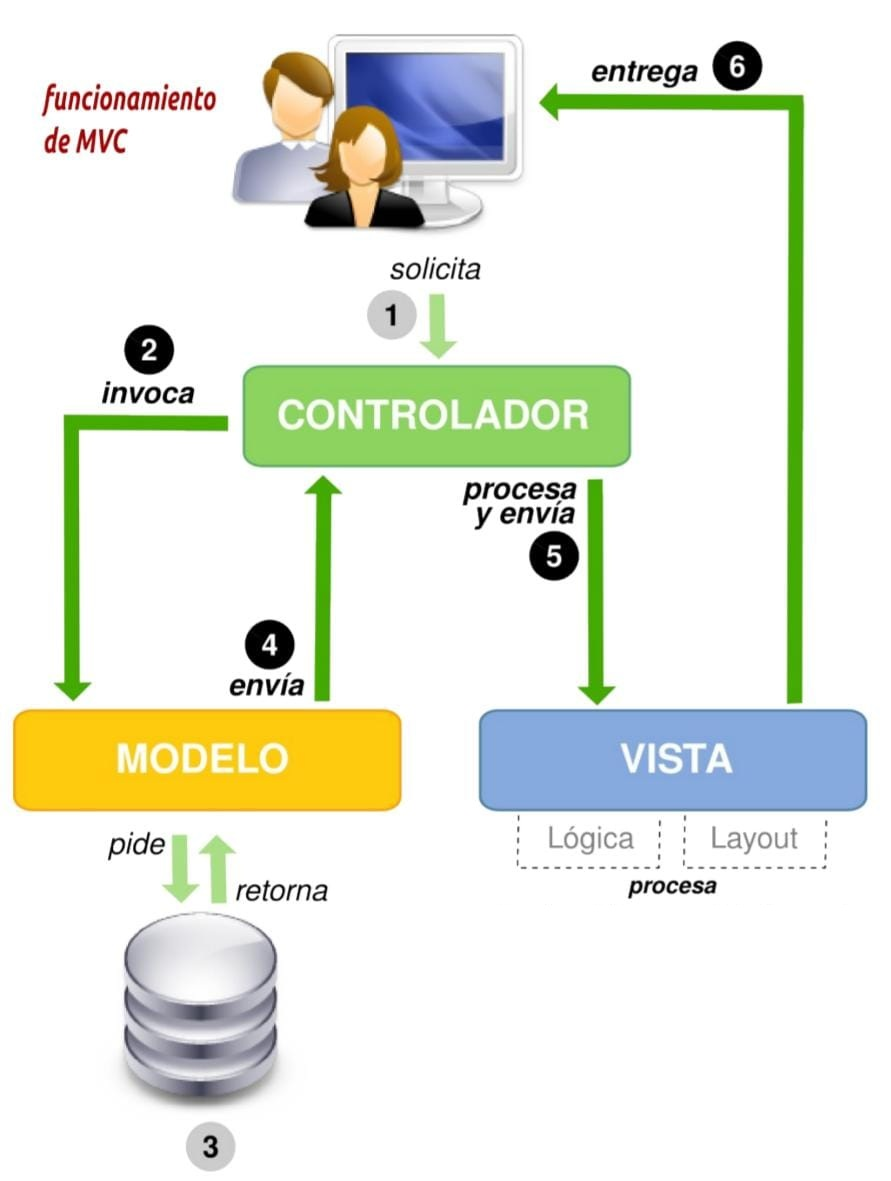
\includegraphics[width=0.5\textwidth]{figuras/patronmvc.png}
    \caption{Patrón de diseño Modelo-Vista-Controlador (MVC)}
    \label{fig:patronmvc}
\end{figure}

\subsection{Arquitectura de una aplicación web}

En el desarrollo de software, las aplicaciones web suelen combinar el modelo cliente/servidor con el patrón MVC. Este enfoque distribuye las responsabilidades del sistema entre el cliente y el servidor, a los que se identifica como \emph{frontend} y \emph{backend} respectivamente. El \emph{frontend} opera como la vista del sistema: presenta la interfaz gráfica, captura las acciones del usuario y emite las peticiones. El \emph{backend} reúne las funciones del controlador y del modelo: atiende las solicitudes entrantes, procesa la lógica del sistema y administra la persistencia de los datos. A continuación, se detallan las características y la organización de cada una de estas partes.

\subsubsection{Frontend}

Al solicitar la aplicación, el navegador descarga un conjunto de archivos que procesa localmente para generar la interfaz. Este proceso se apoya en tres tecnologías complementarias:

\begin{itemize}
    \item HTML (\textit{HyperText Markup Language}, lenguaje de marcado de hipertexto): define la estructura y el contenido del documento. Mediante etiquetas, especifica qué función cumple cada elemento en la interfaz (títulos, bloques de texto, botones o casillas para ingresar datos), organizándolos en un orden lógico que el navegador interpreta para armar la pantalla.
    \item CSS (\textit{Cascading Style Sheets}, hojas de estilo en cascada): controla el aspecto visual y la ubicación de los elementos definidos por HTML. Aplica reglas para definir colores, tipografías, tamaños y espacios, organizando cómo se distribuyen los bloques en la pantalla para que la vista se adapte bien según el tamaño del dispositivo.
    \item JavaScript: es el lenguaje de programación que se ejecuta directamente en el navegador. Mientras que el HTML define qué elementos existen y el CSS define cómo se ven, JavaScript es el encargado de que la página responda a las acciones del usuario: detecta eventos como clics o el envío de un formulario, altera el contenido en pantalla en tiempo real según esa interacción, y se comunica con el servidor para intercambiar información mientras la aplicación está en uso.
\end{itemize}

A medida que una aplicación suma pantallas y funciones, mantener el código fuente en archivos globales vuelve el sistema denso y difícil de ordenar. Para resolver esto, el desarrollo adopta una arquitectura basada en componentes (CBA, \textit{Component-Based Architecture}). En este enfoque, la interfaz se estructura a partir de componentes independientes (Fig.~\ref{fig:componente}), donde cada elemento funciona como una entidad autónoma que reúne su estructura, presentación y lógica asociada.

\begin{figure}[htbp]
    \centering
    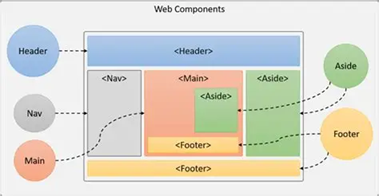
\includegraphics[width=0.5\textwidth]{figuras/componente.png}
    \caption{Características de un componente web}
    \label{fig:componente}
\end{figure}

Bajo este modelo, el código fuente se divide en múltiples archivos modulares que se importan y articulan en un archivo principal. La única relación de dependencia entre componentes se da cuando uno contiene a otro. En esa situación, el componente hijo no puede alterar directamente los datos o estados del padre, sino que solo puede emitir peticiones para solicitar cambios, mientras que el padre sí puede modificar los estados del hijo. Esta estructura ofrece una fácil reusabilidad de elementos, además de garantizar la modularidad y el aislamiento de fallos; es decir, si un componente específico presenta un error, no compromete al funcionamiento del programa en su totalidad.

Para implementar este esquema se utiliza Preact, una biblioteca orientada a componentes que ofrece las mismas capacidades de desarrollo que React pero con una sobrecarga mucho menor. Al prescindir de funciones accesorias innecesarias, el empaquetado final resulta significativamente más liviano, lo que reduce el tamaño de los archivos que el microcontrolador debe almacenar y transferir hacia el navegador al momento de servir la interfaz.

\subsubsection{Backend}

En este desarrollo, el backend adopta una arquitectura en capas basada en el patrón Controlador-Servicio-Repositorio. Esta estructura deriva directamente de MVC ya que, al resolverse la Vista de forma independiente en el cliente web, los Controladores conservan su rol original mientras que el Modelo tradicional se divide en dos capas separadas para diferenciar la lógica de la persistencia de datos.

\begin{itemize}
    \item Controladores (\textit{controllers}): reciben las peticiones que llegan desde el cliente web, extraen los datos de la solicitud y llaman al servicio correspondiente para devolver luego la respuesta. No aplican reglas de funcionamiento ni interactúan con los datos guardados.
    \item Servicios (\textit{services}): representan la parte del Modelo encargada de la lógica del sistema. Reciben los datos procesados por el controlador, aplican las reglas operativas, realizan validaciones y coordinan cuándo consultar o modificar información mediante los repositorios.
    \item Repositorios (\textit{repositories}): representan la parte del Modelo dedicada exclusivamente a los datos y su almacenamiento. Son los únicos que leen y escriben en la base de datos o en la memoria, aislando los detalles de la persistencia del resto del sistema.
\end{itemize}

En este trabajo, estas capas se desarrollaron en C++ junto con el resto del código del sistema embebido, ejecutándose todo dentro del microcontrolador.

\section{Bases de Datos y Persistencia}

\subsection{Conceptos de bases de datos relacionales}

Una base de datos es una colección organizada e integrada de datos almacenados de forma persistente para su posterior consulta y manipulación. Dentro de los distintos paradigmas existentes, el modelo relacional organiza la información en estructuras bidimensionales denominadas tablas (o relaciones), compuestas por filas (registros o tuplas) y columnas (campos o atributos).

Los fundamentos de este modelo se basan en los siguientes conceptos:

\begin{itemize}
    \item Estructura y esquemas: cada tabla posee un esquema definido que determina el tipo de dato que puede almacenar cada columna (numérico, texto, fecha, etc.), garantizando la consistencia del formato.
    \item Claves e integridad relacional: para identificar de forma unívoca cada registro se utiliza una clave primaria (\emph{Primary Key}). La vinculación entre distintas tablas se establece mediante claves foráneas (\emph{Foreign Keys}), lo que permite relacionar entidades sin duplicar información (integridad referencial).
    \item Lenguaje de consulta estructurado (SQL): es el lenguaje formal estándar (\emph{Structured Query Language}) empleado para definir la estructura de los datos, realizar búsquedas mediante filtros, e insertar, modificar o eliminar información de manera declarativa.
    \item Transacciones y propiedades ACID: una transacción es un conjunto de operaciones que se ejecutan como una única unidad lógica. Para garantizar la confiabilidad, los sistemas relacionales implementan las propiedades ACID: Atomicidad (la operación se completa en su totalidad o no se aplica), Consistencia (se respetan todas las reglas e integridad del esquema), Aislamiento (las operaciones simultáneas no interfieren entre sí) y Durabilidad (los cambios confirmados persisten ante fallos o cortes de energía).
\end{itemize}

\subsection{Motores de bases de datos embebidos}

En el desarrollo de software existen dos formas principales de gestionar una base de datos: mediante sistemas basados en un servidor independiente (que atienden peticiones a través de una red) o mediante \textbf{motores embebidos}.

Un motor de base de datos embebido es una biblioteca de software que se integra directamente dentro del mismo código de la aplicación. En este esquema, el motor no se ejecuta como un proceso separado, sino que forma parte del propio ejecutable del sistema.

\textbf{SQLite} es un motor de base de datos relacional embebido de código abierto ampliamente utilizado que implementa el estándar SQL. Sus características teóricas esenciales son:

\begin{itemize}
    \item Arquitectura sin servidor (\emph{Serverless}): los procesos leen y escriben directamente en el soporte de almacenamiento, eliminando la necesidad de configurar, administrar o mantener un servicio en segundo plano.
    \item Almacenamiento en archivo único: la base de datos completa (esquema, tablas, índices y datos) se almacena dentro de un único archivo en el sistema de archivos del dispositivo, lo que simplifica su copia, transporte y respaldo.
    \item Autonomía y portabilidad (\emph{Self-contained}): no depende de bibliotecas externas complejas ni de configuraciones previas en el sistema operativo, permitiendo su funcionamiento en entornos con recursos de memoria y procesamiento acotados.
    \item Cumplimiento transaccional: a pesar de su tamaño compacto, implementa transacciones atómicas que aseguran que los datos no se corrompan ante reinicios o pérdidas de alimentación eléctrica imprevistas.
\end{itemize}